\documentclass{article}

\usepackage[margin=2.5cm]{geometry}

\usepackage[T1]{fontenc} 
\usepackage{mathpazo}

\usepackage[utf8]{inputenc}
\usepackage{amsfonts} 
\usepackage{array} 
\usepackage{enumitem}
\usepackage{tabularx}
\usepackage{graphicx}
\usepackage{fancyhdr}
\usepackage{fancyvrb}
\usepackage{amsmath}
\usepackage{amsthm}
\usepackage[most]{tcolorbox}
\tcbuselibrary{breakable}
\usepackage{float}
\usepackage{listings}  
\usepackage{xcolor}
\usepackage{subfigure}
\usepackage[htt]{hyphenat}
\usepackage{hyperref}
\usepackage{multicol}

%%%%%%%%%%%%%%%%%%%%% BIB %%%%%%%%%%%%%%%%%%%%%%%%%%%%%%%
\usepackage[backend=biber,style=apa,autocite=inline]{biblatex}
\DeclareLanguageMapping{english}{english-apa}
\addbibresource{mem.bib}
%%%%%%%%%%%%%%%%%%%%%%%%%%%%%%%%%%%%%%%%%%%%%%%%%%%%%%%%%

\definecolor{codegreen}{rgb}{.2,0.6,0}
\definecolor{codegray}{rgb}{0.5,0.5,0.5}
\definecolor{codepurple}{rgb}{0.58,0,0.82}
\definecolor{codeblue}{rgb}{0,0.4,0.82}
\definecolor{codeorange}{rgb}{0.94,0.34,0.0}
\definecolor{backcolour}{rgb}{0.95,0.95,0.92}
\definecolor{backcolourgray}{rgb}{0.92,0.92,0.92}
\definecolor{codewhite}{rgb}{1,1,1}

\lstdefinestyle{mystyle}{
    backgroundcolor=\color{backcolourgray},   
    commentstyle=\color{codegreen},
    keywordstyle=\color{codeblue},
    numberstyle=\tiny\color{black},
    stringstyle=\color{codeorange},
    basicstyle=\ttfamily\footnotesize,
    breakatwhitespace=false,         
    breaklines=true,                 
    captionpos=b,                    
    keepspaces=true,                 
    %numbers=left,                    
    numbersep=5pt,                  
    showspaces=false,                
    showstringspaces=false,
    showtabs=false,                  
    tabsize=2,
    extendedchars=true,
    frame=single
    %, basicstyle=\footnotesize
}
\lstset{style=mystyle}

\usepackage{hyperref}
\hypersetup{
    colorlinks=true,
    allcolors=blue,
    %linkcolor=green,
    %filecolor=magenta,      
    %urlcolor=blue,
    %citecolor=blue,
}

\pagestyle{fancy}
\fancyhf{}
\rhead{AI. Practice 2.}
\lhead{Pablo Cuesta Sierra, Álvaro Zamanillo Sáez - G2351, P05}
\cfoot{\thepage}

\usepackage{titlesec}
%\titleformat*{\subsection}{\large\bfseries\color{darkgray}}
%\titleformat*{\subsubsection}{\normalsize\itshape\color{darkgray}}

%\setlength{\parskip}{0.15cm}


%parameters: file, caption, label, scale
\newcommand{\myFigure}[4]{%
    \begin{figure}[H]
        \includegraphics[width=#4\textwidth]{#1}
        \centering
        \caption{#2}
        \label{#3}
    \end{figure}
}

%grey item for enumerate
%\renewcommand{\thesubsubsection}{(\thesubsection.\alph{subsubsection})}
\setcounter{secnumdepth}{4}
\setcounter{tocdepth}{3}
%\newcommand{\question}[1]{\subsection{#1}}
%\newcommand{\subquestion}[1]{\subsubsection{#1}}


\setcounter{section}{0}


\title{\textbf{Artificial Intelligence. Practice 2.}}
\author{\textbf{Pablo Cuesta Sierra, Álvaro Zamanillo Sáez} \\Group 2351. Pair 5.}
%\date{}

\begin{document}

\vspace*{-1.5cm}
{\let\newpage\relax\maketitle}

%\begin{tcolorbox}
\tableofcontents
%\end{tcolorbox}

\pagebreak

\section{Minimax and alpha-beta pruning}

The tests designed and applied to determine the correctness of the implementation are commented in subsection \ref{correctness}.

We have coded the alpha-beta pruning algorithm following exactly the pseudocode provided. The alpha-beta minimax class used follows the template given where the only function to be implemented is \texttt{next\_move()}.  

The code is the following:

\begin{lstlisting}[language=python, caption = Implementation of the alpha beta pruning algorithm,captionpos=t,numbers=left]
    def next_move(
        self,
        state: TwoPlayerGameState,
        gui: bool = False,
    ) -> TwoPlayerGameState:
        """Compute the next state in the game."""
        # NOTE <YOUR CODE HERE>

        alpha, beta = -np.inf, np.inf
        alpha, minimax_successor = self._max_value(
            alpha, 
            beta,
            state,
            self.max_depth_minimax,
        )

        if self.verbose > 1:
            print('{}: [{:.2g}, {:.2g}]'.format(state.board,alpha,beta))

        return minimax_successor
    
    def _min_value(
        self,
        alpha: int,
        beta:  int,
        state: TwoPlayerGameState,
        depth: int,
    ) -> float:
        """Min step of the alpha beta algorithm."""

        minimax_successor = None

        if state.end_of_game or depth == 0:
            beta = min(beta, self.heuristic.evaluate(state))
        else:
            for successor in self.generate_successors(state):
                if self.verbose > 1:
                    print('{}: [{:.2g}, {:.2g}]'.format(state.board,alpha,beta))

                successor_alpha, _ = self._max_value(
                    alpha,
                    beta,
                    successor,
                    depth - 1,
                )
                if (successor_alpha < beta):
                    beta = successor_alpha
                    minimax_successor = successor
                if (alpha >= beta):
                    break

        if self.verbose > 1:
            print('{}: [{:.2g}, {:.2g}]'.format(state.board,alpha,beta))

        return beta, minimax_successor

    def _max_value(
        self,
        alpha: int,
        beta:  int,
        state: TwoPlayerGameState,
        depth: int,
    ) -> float:
        """Max step of the alpha beta algorithm."""

        minimax_successor = None

        if state.end_of_game or depth == 0:
            alpha = max(alpha, self.heuristic.evaluate(state))
        else:
            for successor in self.generate_successors(state):
                if self.verbose > 1:
                    print('{}: [{:.2g}, {:.2g}]'.format(state.board,alpha,beta))

                successor_beta, _ = self._min_value(
                    alpha,
                    beta,
                    successor,
                    depth - 1,
                )
                if (successor_beta > alpha):
                    alpha = successor_beta
                    minimax_successor = successor
                if (alpha >= beta):
                    break

        if self.verbose > 1:
            print('{}: [{:.2g}, {:.2g}]'.format(state.board,alpha,beta))

        return alpha, minimax_successor
\end{lstlisting}

The \texttt{\_max\_value()} function is the function that is applied to MAX nodes, and \texttt{\_min\_value()} to MIN nodes. Each of these two functions calls the other, because each MIN node has successors which are MAX nodes, and vice versa. The recursion ends when a node is a leaf (end of the game), or the maximum depth is reached. In that case the algorithm returns the evaluation function in that node. \texttt{\_max\_value()} and \texttt{\_min\_value()} have the same logic but with the roles of alpha and beta exchanged (except for the prune condition (lines 49 \& 84) which is, as expected, the same for MIN and MAX nodes).

\subsection{Testing alpha-beta pruning correctness with the `simple game tree'}\label{correctness}

We will now follow the instructions provided to check correctness with the ``simple game tree''.

\myFigure{./aditional/simple_game_tree}{``Simple game tree''.}{simple_game_tree}{.5}

\subsubsection{Manually applying minimax to the tree }

\myFigure{./aditional/manual_minimax}{Minimax.}{manual_minimax}{1}

\subsubsection{Applying the coded minimax algorithm to the tree}

\begin{lstlisting}[captionpos=t,caption=Minimax execution with the `simple game tree'.]
Let's play SimpleGameTree!

A

It is the turn of player 'Minimax 1' [Player 1].

A: -inf
B: inf
E: 4
B: 4
F: 3
B: 3
A: 3
C: inf
G: -inf
K: 2
G: 2
L: 1
G: 2
C: 2
H: 5
C: 2
A: 3
D: inf
I: 5
D: 5
J: -inf
M: 4
J: 4
N: 2
J: 4
O: 6
J: 6
P: 1
J: 6
D: 5
A: 5

Game state before move:

A

Minimax value = 5

Player 'Minimax 1' [Player 1] moves AD.

\end{lstlisting}

The execution goes exactly as expected.

\subsubsection{Manually applying alpha-beta minimax to the tree }

\myFigure{./aditional/manual_ab}{Alpha-beta minimax.}{manual_ab}{1}

\subsubsection{Applying the coded alpha-beta minimax algorithm to the tree}

\begin{lstlisting}[captionpos=t,caption=Alpha beta minimax execution with the `simple game tree'.]
Let's play SimpleGameTree!

A

It is the turn of player 'Minimax + alpha-beta 1' [Player 1].

A: [-inf, inf]
B: [-inf, inf]
E: [4, inf]
B: [-inf, 4]
F: [3, 4]
B: [-inf, 3]
A: [3, inf]
C: [3, inf]
G: [3, inf]
K: [3, 2]
G: [3, inf]
L: [3, 1]
G: [3, inf]
C: [3, 3]
A: [3, inf]
D: [3, inf]
I: [5, inf]
D: [3, 5]
J: [3, 5]
M: [3, 4]
J: [4, 5]
N: [4, 2]
J: [4, 5]
O: [4, 5]
J: [5, 5]
D: [3, 5]
A: [5, inf]
A: [5, inf]

Player 'Minimax + alpha-beta 1' [Player 1] moves AD.
        
\end{lstlisting}

We did not get it in our first try, mainly because of differently named variables, not initializing some values, etc. But the first successful execution (no syntax errors and no uninitialized variables) performed as expected in figure \ref{manual_ab}. 

Finally, to make sure that our implementation is correct, we have executed several Othello matches using deterministic players and starting from the same positions, and we have checked that the entire games were the same regardless of the minimax algorithm used. 

\subsection{Verifying pruning performance}\label{intro:performance}

To verify that pruning is working, we will now make a small time report, where we will measure the execution of Othello matches using minimax and alpha-beta pruning at different depths.

In order to test this, we have written a python script (\emph{time\_minimax.py}) that takes as argument the depth at which the match will be played and the strategy to use (either ordinary minimax or alpha-beta minimax). This script will create two players with this strategy and measure the time it takes to play a single match. 

We have used the \textit{timeit} package, as suggested.

\begin{lstlisting}[language=python,captionpos=t,caption=Match time measure]
    start_time = timeit.default_timer()
    match.play_match()
    end_time = timeit.default_timer()

    print("Time:", end_time - start_time)
\end{lstlisting}

In order to get a good comparison between the two algorithms, we have compared them at depths 2, 3 and 4. Our testing script (\emph{time\_minimax.sh}) executes 20 matches with each algorithm and each (maximum) depth, after which the time mean (in seconds) is calculated for each algorithm and depth. In order to get a computer-independent
measure, we have computed with each depth the speedup of alpha-beta pruning with respect to regular minimax:

    $$\text{Speedup}=\frac{\text{Minimax time mean}}{\text{Alpha-beta pruning time mean}}$$

It is worth mentioning, that measuring time is always a delicate task as the results not only depend on the programs being run, but also on the machine where the tests are carried out and the tools used. Therefore, all the results provided here must be taken as a reference of improvement between two algorithms rather than the performance of any of them individually.


\begin{lstlisting}[language=bash, caption = Complete description of the tests carried out (\emph{time\_minimax.sh}),captionpos=t]
#!/bin/bash

DEPTHS=(2 3 4)
REP=20
TAB="\t"
DECIMALS=4

DAT_DIR="../results"
MEM_DIR="../mem"

TIME_SCRIPT="../scripts/time_minimax.py"
EXECUTE="python3 ${TIME_SCRIPT}"

TMP_FILE="${DAT_DIR}/time_tmp.dat"
TMP_FILE2="${DAT_DIR}/time_tmp2.dat"
OUT_FILE="${DAT_DIR}/time_minimax_output.dat"
LATEX_TABLE_FILE="${MEM_DIR}/aditional/times_table.tex"
EXEC_LATEX_TABLE_SCRIPT="python3 latex_table.py"

mkdir -p ${DAT_DIR}
rm -f ${TMP_FILE} ${TMP_FILE2} ${OUT_FILE}

echo "Running minimax vs alpha-beta timing: ${REP} repetitions for depths {${DEPTHS[@]}}"

for depth in ${DEPTHS[@]}; do
    echo "  Doing depth $depth"
    for ((j = 1; j <= REP ; j += 1));do
        echo "    Iteration $j"
        time_minimax=$(${EXECUTE} $depth "minimax"    | grep -i "time" | awk '{print $2}' )
        time_alpha_beta=$(${EXECUTE} $depth "alpha-beta" | grep -i "time" | awk '{print $2}' )
        echo "minimax $depth $time_minimax" >> ${TMP_FILE}
        echo "alpha_beta $depth $time_alpha_beta" >> ${TMP_FILE}
    done
done

cat ${TMP_FILE} | tr "." "," > ${TMP_FILE2} # for awk 

# calculate the means and the ratio
echo -e "Max depth${TAB}Minimax mean${TAB}Alpha-beta mean${TAB}Speedup" >> ${OUT_FILE}

for depth in ${DEPTHS[@]}; do
    minimax_mean=$(grep -w "minimax $depth" ${TMP_FILE2} | awk '{ times += $3; n++ } END { printf "%s", times/n }')
    alpha_beta_mean=$(grep -w "alpha_beta $depth" ${TMP_FILE2} | awk '{ times += $3; n++ } END { printf "%s", times/n }')
    minimax_mean=$(echo $minimax_mean | tr "," ".")
    alpha_beta_mean=$(echo $alpha_beta_mean | tr "," ".")
    speedup=$(echo "scale=${DECIMALS};$minimax_mean/$alpha_beta_mean" | bc)
    echo -e "${depth}${TAB}${minimax_mean}${TAB}${alpha_beta_mean}${TAB}${speedup}" >> ${OUT_FILE}
done

rm -f ${TMP_FILE2}

echo "Writing latex table to file ${LATEX_TABLE_FILE}..."
${EXEC_LATEX_TABLE_SCRIPT} ${OUT_FILE} >> ${LATEX_TABLE_FILE} 

\end{lstlisting}

\subsubsection{With a constant heuristic }\label{table:constant_heuristic}

We will first measure matches played using a constant evaluation function. This heuristic takes the same time to calculate in every case (almost none). The measurements are the following:

\begin{table}[h!]
    \centering
    \begin{tabular}{|r|r|r|r|}
  % ordenador de Pablo
\hline
   Max depth &   Minimax mean (s) &   Alpha-beta mean (s) &   Speedup
 \\
\hline
           2 &        1.786   &           1.474   &     1.212 \\
           3 &       10.341   &           3.581   &     2.887 \\
           4 &       73.964   &          11.720   &     6.311 \\
\hline
\end{tabular}

    \caption{Constant heuristic tests.}
    \label{table:cte}
\end{table}

At depth 2, the difference is significant, but the power of pruning can be better appreciated at higher depths. As can be seen, at depth 4, alpha-beta pruning is more than 6 times faster than minimax. This is a very specific case and would make no sense in practice as the heuristic used does not provide any information about the states evaluated. However, we have included this example to illustrate how the performance of alpha pruning depends on the order in which nodes are explored. With the constant heuristic, the ``best'' nodes are explored first and, therefore, a lot of pruning is carried out.

In the next image, we illustrate the pruning done for a tree with a branching factor of 3 and depth 3.

\myFigure{./images/constant_b3_d4.png}{Alpha-Beta execution with a constant heuristic}{}{.9}

As can be seen, this heuristic yields the best possible performance out of the alpha-beta algorithm, as the highest possible amount of pruning that can be made is actually done (starting with initial values $[-\infty,\infty]$); thus, it is not to be expected that the speedups of alpha-beta pruning with respect to minimax are as high when using any other (non-constant) heuristic.

\subsubsection{With a random heuristic}\label{table:random_heuristics}

This time, we are going to use an heuristic that returns a random number. The proportion of nodes pruned will be closer to the one obtained when using a generic heuristic. Although the matches are not exactly the same (because of the random heuristic), we are making several repetitions of the matches, as commented in \ref{intro:performance}, so this fact should not be a great issue when comparing minimax with alpha-beta.

\begin{table}[h!]
    \centering
    \begin{tabular}{|r|r|r|r|}
    \hline
       Max depth &   Minimax mean &   Alpha-beta mean &   Speedup
     \\
    \hline
               2 &        3.336 &           1.999 &     1.168 \\
               3 &       31.983  &           19.828 &     1.613 \\
               4 &      223.873   &          70.267  &     3.186 \\
    \hline
    \end{tabular}
    
    \caption{Tests carried out with a random heuristic.}
    \label{table:our}
\end{table}

Looking at the table, one can observe that the speedup obtained for depth 4 is half of the one obtained with a constant heuristic. Once again, this is due to the order in which the best nodes are expanded. With the random heuristic, we have no guarantee of expanding the best nodes early. As a result, the pruning performed will be less than in the previous case.

\subsubsection{With one of our heuristics }\label{table:our_heuristic}

Finally, here we used the heuristic explained in \ref{winner}. This heuristic is far more sophisticated than a constant (or random) heuristic, as it has to make some calculations with the characteristics of the board in each state of the game. Therefore, absolute times are expected to be much higher than in the previous tests. 

On the other hand, the proportion of nodes pruned can be assumed to be similar to what we would get using a random heuristic (definitely lower than with a constant heuristic \ref{table:constant_heuristic}). So the amount of nodes traversed and evaluated this time can be compared to the case of a random heuristic. However, executing our heuristic consumes more time than generating a random number, thereby the explanation of why the speedup is greater with one of our heuristics in contrast to the random heuristic:


\begin{table}[h!]
    \centering
    \begin{tabular}{|r|r|r|r|}
\hline
   Max depth &   Minimax mean &   Alpha-beta mean &   Speedup
 \\
\hline
           2 &        2.50623 &           1.97239 &     1.2706 \\
           3 &       20.4784  &           9.16699 &     2.2339 \\
           4 &      407.619   &          86.1799  &     4.7298 \\
\hline
\end{tabular}

    \caption{Tests carried out with our heuristic.}
    \label{table:our}
\end{table}

\pagebreak

Asymptotically, that is, for big enough depths, the complexity of (regular) minimax is $\mathcal{O}(b^d)$, whereas that of alpha-beta is $\mathcal{O}(b^{d/2})$, where $b$ is the branching factor (constant on average, for Othello games), and $d$ is the depth used for the algorithm~\autocite{russellnorvig}. Therefore, the speedup should follow a function that is $\mathcal{O}(b^{d/2})$ -- exponential, -- with the very small amount of data that we have, this is compatible with our results.

\section{Heuristic}

For the design of our heuristic we began by doing a research to learn the features we should take into account in the heuristic.  

The winner of the game is the one who ends with the most number of coins, therefore one would think (naively) that maximizing coins is a good strategy. Indeed, as stated in~\textcite{washington1}, this strategy was used by the first Othello programs but "failed miserably". This gave us our first clue to weigh ``low'' the coin count. 

On the other hand, several documents and books~\autocite{paradigms} emphasized the importance of mobility and stability. So with these few ideas on mind, we started to develop our first heuristics.

Now, we proceed to explain the process of developing the different heuristics we presented to the tournaments, as well as the conclusions we reached based on the performance of them. In general, our design process was gradual and consisted on improving two heuristics which differ in the way the tackle the problem of evaluating states.

\subsection{Initial Heuristics}

The following heuristics are simple and take into account a single aspect of the game. We will later combine these in order to get more complete heuristics.

\subsubsection{Coin difference heuristic }

This is the first obvious heuristic, simply consists on the difference of coins divided by the total amount of coins in the board~\autocite{washington1}:

$$\text{(Coin difference heuristic)} = 100 \times\frac{\text{(Max coins)}-\text{(Min coins)}}{\text{(Max coins)}+\text{(Min coins)}}$$

\subsubsection{Corner difference }

This is the second obvious heuristic, which takes into account the only pieces in the board that are always stable (cannot be captured): the corners~\autocite{washington1}.

$$\text{(Corner difference heuristic)} = 100\times\frac{\text{(Max corners)}-\text{(Min corners)}}{\text{(Max corners)}+\text{(Min corners)}}$$

\subsubsection{Simple evaluation function}

While we were developing the first heuristic, we needed another heuristic to compete against. This heuristic is basically random and therefore, our designs should beat it almost every time. This was a provided heuristic.

\begin{lstlisting}[language=python, caption = Simple evaluation function,captionpos=t]
def simple_evaluation_function(state: TwoPlayerGameState) -> float:
    """Return a random value, except for terminal game states."""
    state_value = 2*np.random.rand() - 1

    if state.end_of_game:
        scores = state.scores
        # Evaluation of the state from the point of view of MAX

        assert isinstance(scores, (Sequence, np.ndarray))
        score_difference = scores[0] - scores[1]

        if state.is_player_max(state.player1):
            state_value = score_difference
        elif state.is_player_max(state.player2):
            state_value = - score_difference
        else:
            raise ValueError('Player MAX not defined')

    return state_value
\end{lstlisting}

\subsubsection{Using a weighted board}\label{static_board}

One idea repeated all over, was employing a weighted board that takes into account how good a position is~\autocite{washington1}. In contrast to just taking account number of coins, this approach considers the topological characteristics of Othello: it penalizes tiles adjacent to corners (because they allow the capture of the corner) while it encourages capturing a corner (tiles with the maximum value). 

We found three different weighted boards (following listing). We tried using the different boards against our other heuristics (\ref{scripts_compare})  to see if any worked considerably better than the rest but all of them performed similar. 



% WEIGHTED BOARDS
\begin{lstlisting}[captionpos=t,language=python,linewidth=1\textwidth,caption={Our 3 weighted boards: from \cite{washington1} (the first two), and \cite{CaseStudy} (the third).}]
    weights1 = [
        [ 4, -3,  2,  2,  2,  2, -3,  4],
        [-3, -4, -1, -1, -1, -1, -4, -3],
        [ 2, -1,  1,  0,  0,  1, -1,  2],
        [ 2, -1,  0,  1,  1,  0, -1,  2],
        [ 2, -1,  0,  1,  1,  0, -1,  2],
        [ 2, -1,  1,  0,  0,  1, -1,  2],
        [-3, -4, -1, -1, -1, -1, -4, -3],
        [ 4, -3,  2,  2,  2,  2, -3,  4]
    ]
    weights2 = [
        [100,-10, 11,  6,  6, 11,-10,100],
        [-10,-20,  1,  2,  2,  1,-20,-10],
        [ 10,  1,  5,  4,  4,  5,  1, 10],
        [  6,  2,  4,  2,  2,  4,  2,  6],
        [  6,  2,  4,  2,  2,  4,  2,  6],
        [ 10,  1,  5,  4,  4,  5,  1, 10],
        [-10,-20,  1,  2,  2,  1,-20,-10],
        [100,-10, 11,  6,  6, 11,-10,100],
    ]
    weights3 = [
        [120,-20, 20,  5,  5, 20,-20,120],
        [-20,-40, -5, -5, -5, -5,-40,-20],
        [ 20, -5, 15,  3,  3, 15, -5, 20],
        [  5, -5,  3,  3,  3,  3, -5,  5],
        [  5, -5,  3,  3,  3,  3, -5,  5],
        [ 20, -5, 15,  3,  3, 15, -5, 20],
        [-20,-40, -5, -5, -5, -5,-40,-20],
        [120,-20, 20,  5,  5, 20,-20,120],
    ]
    \end{lstlisting}\label{weighted_boards}

%\pagebreak

Our first heuristic used always the same weighted board and gave a result according to the weighted sum of \textit{MAX}'s coins minus \textit{MIN}'s weighted score.

\begin{lstlisting}[language=python, caption = Weighting the board,captionpos=t]
def static_weights_player(board: dict, player_label: Any, weights) -> float:
    return sum(
            weights[key[0] - 1][key[1] - 1]
            for key in board.keys() if (board[key] == player_label)
        )

def static_weights_heuristic(state: TwoPlayerGameState, weights) -> float:
    ''' 100 * (sum of p1's weights - sum of p2's weights) / (# of coins in the board) '''
    return 100 *                                                                       \
            (static_weights_player(state.board, state.player1.label, weights)          \
           - static_weights_player(state.board, state.player2.label, weights)) / len(state.board) 
\end{lstlisting}


This approach of using a static board gave quite acceptable results but presented a problem. While \texttt{coin\_diff} and \texttt{corner\_diff} are proportions (multiplied by 100), and take values in $[-100,100]$, the result of weighting the board varies significantly through the match and it was not clear how to combine efficiently this value with the ones given by \texttt{coin\_diff} and \texttt{corner\_diff}. The option we chose is to divide the weights by the number of coins present in the board, which makes this heuristic closer to proportion kind of heuristic we are looking for.


\subsubsection{Penalizing tiles adjacent to corners}

In order to penalize giving a corner to the opponent, we have made a function that detects when the opponent has direct access to the corner in the next move. That is to say, we penalize the tile adjacent to the corner if the corner is not captured and also if the opponent has a coin in the tile next to the adjacent tile. This penalization allowed the heuristic to look ahead one extra level in depth when considering the control of corners compared to just using \textit{corner\_diff} for the same task. 


\begin{lstlisting}[language=python, caption = Penalize giving corners,captionpos=t]
    def dont_give_corner(state: TwoPlayerGameState,player1_label,player2_label) -> float:
        board=state.board
        #Dictionary indexed by the corner:
        #  | val[1]       val[5]
        #  | val[0] val[4]
        #  | key    val[2] val[3]
        #   -----------------------

        corners={(1,1):[(1,2),(1,3),(2,1),(3,1),(2,2),(3,3)],
                (1,8):[(1,7),(1,6),(2,8),(3,8),(2,7),(3,6)],
                (8,1):[(7,1),(6,1),(8,2),(8,3),(7,2),(6,3)],
                (8,8):[(7,8),(6,8),(8,7),(8,6),(7,7),(6,6)]}

        penalization = 0
        for (corner, values) in corners.items():
            if corner in board.keys():  # The corner is already taken
                continue

            for i in range(3):
                try:
                    # Player 2 has access to the corner
                    if   board[values[0+i]] == player1_label and board[values[1+i]] == player2_label:
                        penalization += 1
                    # Player 1 has access to the corner
                    elif board[values[0+i]] == player2_label and board[values[1+i]] == player1_label:
                        penalization -= 1
                except:
                    continue
        return penalization

\end{lstlisting}

This function returns the number of corners that \textit{player2} could capture with the current board situation minus those that \textit{player1} could capture. This will later be used by the heuristics to penalize the evaluation of the board.

\subsection{Comparing heuristics}

At this point, we were developing several heuristic and we needed to decide which one performed the best. In order to make a ``based'' decision we implement several features that allowed us to carry out test.

\subsubsection{Generation of random boards}

All our heuristics are deterministic, therefore, a match between two of them will always lead to the same result for a given board. On the other hand, running matches from an initial board is quite slow. Based on those two ideas, we created a collection of random boards by playing \textit{random} vs \textit{random} a limited number of moves. This way, we could test our heuristics starting from different stages of the game. By varying the number of moves executed by each random-player we could generate a collection of boards with an almost starting position, intermediate position or with an ending position. (The generated boards are in \emph{random\_boards.py}.)

Each match of our tournament was carried out with a random pick from that collection of boards. 

\subsubsection{Scripts}\label{scripts_compare}

In order to compare heuristics, we wrote a simple script that allowed us to face two heuristics and save the output to a file. Then with a second script, we could decide how many heuristics to face so we could leave the computer running the matches all night and then see the results the next morning and make the decisions on whether a ponderation gave better results.

\begin{lstlisting}[language=bash, caption = Comparing two heuristics,captionpos=t]
#!/bin/bash

RES_DIR="../results/"

REP=30

mkdir -p ${RES_DIR}

COMMAND="python3 ../scripts/demo_tournament.py"
OUTPUT="${RES_DIR}comp.dat"

touch $OUTPUT

echo -e "Running $1 vs $2 -- $REP rounds"

t1=0
t2=0
for ((j = 0 ; j < REP ; j += 1));do
    op1=( $(${COMMAND} $1 $2 | grep 'opt1' | awk '{print $2}') )
    op2=$((2-$op1))

    t1=$(echo $(($t1+$op1)) )
    t2=$(echo $(($t2+$op2)) )

    echo -e " $j Result $1 vs $2: $op1 : $op2  Total so far: $t1 : $t2"
done

echo -e "$1 vs $2:  $t1 $t2 " >> $OUTPUT
echo -e "   " >> $OUTPUT    
\end{lstlisting}

\subsection{More advanced heuristics}

\subsubsection{Frontiers}

A key feature that we had not taken into account until this moment was mobility. In general, it is recommended to maximize your own mobility while minimizing your opponent's~\autocite{reversistrategy}.

One way of taking into account mobility is by the concept of frontiers: a frontier is a coin that has unoccupied tiles adjacent to it~\autocite{reversistrategy}. Your opponent can only place their disks in empty tiles next to your own, so by reducing your number of frontier disks, you are reducing the potential moves of your opponent.

(Disclaimer: the provided function \texttt{\_get\_valid\_moves} does calculate the exact number of valid moves while using frontiers gives only an approximation. However, calculating the exact number of moves is quite more expensive in time terms and, on the other hand, it does not provide much better results).

\begin{lstlisting}[language=bash, caption = Frontiers detection code,captionpos=t]
    def unoccupied(self, i,j,board) -> bool:
    '''whether position i,j of the board array is occupied, False if it is out of bounds'''
        if (i < 0) or (j < 0) or (i >= 8) or (j >= 8):
            return False 
        return board[i][j] == '.'

    def is_frontier(self, i,j, board) -> bool:
        if (i,j) in [(0,0),(0,7),(7,0),(7,7)]: 
            return False
        surrounding = [
                (i-1,j-1),(i  ,j-1),(i+1,j-1),
                (i-1,j  ),          (i+1,j  ),
                (i-1,j+1),(i  ,j+1),(i+1,j+1)
        ]
        return any(self.unoccupied(i,j,board) for (i,j) in surrounding)

    def frontiers_player(self, state: TwoPlayerGameState, label: Any) -> float:
        board_arr = from_dictionary_to_array_board(state.board, 8, 8)
        player_pieces = [
            (j-1,i-1) for (i,j) in state.board.keys() if state.board[(i,j)] == label
        ]
        return sum(self.is_frontier(i,j, board_arr) for (i,j) in olayer_pieces)

    def frontiers(self, state: TwoPlayerGameState) -> float:
        p1 = self.frontiers_player(state, state.player1.label)
        p2 = self.frontiers_player(state, state.player2.label)
        if p1 or p2:
            return 100*(p2-p1)/(p1+p2)
        else:
            return 0
\end{lstlisting}

\subsubsection{Dynamic Board}\label{dynamic_heuristic}

One of the weaknesses of the static  board is that assumes some tiles are always a bad choice. In other words, it does not consider the actual state of the board. Our approach to improve this heuristic was to partially reevaluate the board. We decided to limit this reevaluation to the edges for two reasons: first of all, edges are key tiles due to their potential stability, and secondly, reevaluating the whole board (in a coherent way) requires strong understanding of the Othello game, which we obviously lack.

The reevaluation follows this logic: once a player has captured a corner, tiles adjacent to that corner are no longer bad positions. Indeed, they become stable coins and therefore, should be weighted positively. Our new heuristic reconsiders weights from the corner in the edges direction as long as the player controls a chain to the corner.

We include the functions used to reevaluate: 
\begin{itemize}
    \item \texttt{weights\_modify} is the wrapper function that iterates over the four corners. We stored in a dictionary, indexed by corners positions, the expansion directions for each corner. 
    \item \texttt{edge\_weights} is the function that actually changes the weights.
\end{itemize}

\begin{lstlisting}[language=python, caption = Functions to reevaluate,captionpos=t]
    def weights_modify(self, 
                       weights: list[list[int]], 
                       state: TwoPlayerGameState) -> list[list[int]]:
        board=state.board
        corners=[(1,1),(1,8),(8,1),(8,8)]
        my_weights=copy.deepcopy(weights)
        taken_corners=list(set(corners) & set(board.keys()))

        corner_weight=weights[0][0]
    
        directions={(1,1): [(1,0),(0,1)],
                    (1,8): [(1,0),(0,-1)],
                    (8,1): [(-1,0),(0,1)],
                    (8,8): [(-1,0),(0,-1)]}

        for corner in taken_corners:
            self.edge_weights(weights=my_weights, 
                            state=state, 
                            corner=corner,
                            directions=directions[corner],
                            player_label=board[corner],
                            new_weight=corner_weight
                        )
        return my_weights

    def edge_weights(self,
                     weights,
                     state: TwoPlayerGameState,
                     corner, 
                     directions,
                     player_label,
                     new_weight):
       board=state.board

       for dir in directions:
            pos=(corner[0]+dir[0],corner[1]+dir[1])

            while pos in board.keys() and board[pos] == player_label:
                weights[pos[0]-1][pos[1]-1]=new_weight
                pos=(pos[0]+dir[0],pos[1]+dir[1])

\end{lstlisting}


This heuristic was used in the second tournament and, while for intermediate matches performed quite well, for initial positions it was not so good. A possible explanation is that this heuristic rewards considerably the edges; however, at the beginning of the game interior stability (as mentioned in~\textcite{othellus}) is a key aspect; but this heuristic tends to expand towards the edges which contradicts this principle.


\subsection{Tournaments and evolution of our heuristics}

For the tournaments, we had to combine the previous heuristics in order to get a more complete evaluation of the game state, while we discard some options that did not performed as expected.

\subsubsection{First tournament }

Out heuristics for this tournament were of two types: the first, a combination of coin difference, corner difference and frontiers; and the second, the dynamic board heuristic (commented in \ref{dynamic_heuristic}). The first one had the best results (the two variations were in position 2 and 3 in the tournament).

\pagebreak

\begin{lstlisting}[language=python,captionpos=t, caption=Tournament 2 -- our best (most successful) heuristic.]
    def utility(self, state: TwoPlayerGameState) -> float:
        return  0.2 * self.coin_diff(state)                  \
              + 0.4 * self.corner_diff(state)                \
              + 0.4 * self.frontiers(state)
\end{lstlisting}\label{winner}

Something important to note is that this tournament only consisted of matches beginning in an intermediate stage of the game. Therefore, we did not have any information regarding the performance of our heuristics from other starting positions.

\subsubsection{Second tournament }

The second tournament consisted of matches from three different stages: an initial one, an intermediate one and a final position. 

It was just two days after the first one and, as our heuristics had done well in the first one, we maintained the best one, and decided to experiment a little with the others.

The result of this tournament was quite interesting because while the dynamic board and the frontiers version performed quite well for intermediate boards, they obtained average results for initial boards.

\myFigure{./images/tournament2.png}{Results of 2nd tournament (our heuristics are named \texttt{cz\_solution*})}{tour2}{.8}

The conclusion we reached is that we had to differentiate between stages of the game and use different heuristics for each part. In general a game can be divided into an initial phase (that lasts for the 12 first moves in average), the mid-game and end game. Because the tournaments were not carried out from the very beginning, we decided to only consider two stages: mid-game and end-game.


\subsubsection{Third tournament }

As commented above, the conclusion we reached after the second tournament was to use different heuristics for different stages of the game.

For the late game, we did not change the heuristics because the results obtained so far in the tournaments did not encourage us to do so. However, for the mid game, we decided to use static weight boards to encourage the control of the center. The three submitted heuristics differ in the definition of mid-game and late-game. In other words, the only difference between all of them was the numbers of moves that were played with the static weight heuristic. Also, one of the 3 heuristics used one board with static weights for the start and mid-game, and the other two used another one. This way we could adjust for the next tournament according to which static weights board provided better results.

\begin{figure}[h!]
    \centering
    \begin{tabular}{c}
    \begin{lstlisting}[language=python,linewidth=0.5\textwidth]
    weights1 = [
        [4000, -2,  3,  2,  2,  3, -2,4000],
        [  -2,-60, -1, -1, -1, -1,-60,  -2],
        [   3, -1,  2,  1,  1,  2, -1,   3],
        [   2, -1,  1,  1,  1,  1, -1,   2],
        [   2, -1,  1,  1,  1,  1, -1,   2],
        [   3, -1,  2,  1,  1,  2, -1,   3],
        [  -2,-60, -1, -1, -1, -1,-60,  -2],
        [4000, -2,  3,  2,  2,  3, -2,4000]
    ]
    weights2 = [
        [100,-10, 11,  6,  6, 11,-10,100],
        [-10,-20,  1,  2,  2,  1,-20,-10],
        [ 10,  1,  5,  4,  4,  5,  1, 10],
        [  6,  2,  4,  2,  2,  4,  2,  6],
        [  6,  2,  4,  2,  2,  4,  2,  6],
        [ 10,  1,  5,  4,  4,  5,  1, 10],
        [-10,-20,  1,  2,  2,  1,-20,-10],
        [100,-10, 11,  6,  6, 11,-10,100],
    ]
        \end{lstlisting}
    \end{tabular}
    \caption{Our 2 weighted boards for the first stage of the game in third tournament.}\label{weighted_boards2}
\end{figure}

\pagebreak

Furthermore, we modified the weighted board heuristic so that it returns the following:

\begin{lstlisting}[language=python, caption = Weighting the board,captionpos=t]
    def static_weights_player(board: dict, player_label: Any, weights) -> float:
        return sum(
                weights[key[0] - 1][key[1] - 1]
                for key in board.keys() if (board[key] == player_label)
            )    
    def static_weights_heuristic(state: TwoPlayerGameState, weights) -> float:
        ''' (sum of p1's weights - sum of p2's weights) '''
        return (static_weights_player(state.board, state.player1.label, weights)      \
               -static_weights_player(state.board, state.player2.label, weights))
\end{lstlisting}

We no longer try to make the approximation to a proportion that we explained at the end of \ref{static_board}, this new version just returns the difference of weights between the players. The explanation for this is that we no longer combine it with other heuristics, so there is no need to make it proporiton-like. This way, we save some multiplications and divisions.

To sum up, our heuristics had the following schema:

\[  h(n)=
    \begin{cases}
        \text{static\_weights}(n) & \text{Number of coins in board}\leq \text{threshold} \\
        \text{frontiers\_heuristic}(n) & \text{Number of coins in board} > \text{threshold} \\
    \end{cases}
\]
\

where frontiers\_heurstic is the one presented in (\ref{winner}) and threshold $\in \{25,35,45\}$ (for each heuristic submitted we change the threshold).

\subsubsection{Fourth tournament}\label{t4}

The results of the third tournament were similar to those of the second. That is to say, our heuristics were in the top 10 when it comes to intermediate and final starting positions, whereas they descend to percentile 70 for initial positions. 

However, with the inclusion into the tournament of the last board: from the starting position of the game, our heuristics climbed back up in the ranking, and one of them reached position 6 in the tournament.

As we commented before, the third tournament heuristics were the same as the one in \ref{winner} at the end of the game (from move 25-35 onwards), and they had the static weights boards heuristic with different boards at the start of the game. Therefore, we took the heuristic that performed best in this tournament, and made small modifications for the last tournament. We will discuss them in detail in \ref{final_heuristics}

\section{Final Considerations}

\subsection{Othello compared to chess}

None of our heuristics take into account which player is going to make the next move; that is to say, a same board is evaluated the same indepently of who makes the next move. 

In other games, like chess, this would make no sense at all. Take for instance the following board configuration and let white be MAX. If white moves, it will be checkmate, so any heuristic should mark this state with a high score for white. However, if black moves, quite the opposite should happen (black wins, and the heuristic should evaluate high for black). The same reasoning can be applied to boards where two pieces are faced, so depending on who moves, either piece is the one threatened.

\myFigure{./images/tablero1.png}{Chess state example}{tablero1}{0.4}

It is true that for some configurations of Othello boards near to the end of the game, if both players have a similar number of coins, the fact of which player moves could be decisive in the outcome of the match. However, this situations are quite specific and, in general, one could say that it is not needed to know which player makes the move to evaluate a state. In fact, none of the heuristics we found when researching took this aspect into account.


\subsection{Our final heuristics}\label{final_heuristics}

As explained in \ref{t4}, these heuristics are variations of the one that did very well (position 6) in tournament 3. The first heuristic is the same as that one, which used the weighted board at the beginning of the game (first 40 moves), and the heuristic from \ref{winner} at the end.

The second heuristic is the same, with the slight difference that the initial heuristic is used until the 25th move instead of the 40th.

The last heuristic is the same as the first one, but it includes in both the starting and ending stages of the game the heuristic from the Reversi class: \texttt{\_choice\_diff()}. This heuristic measures the differences in mobility of the two players. As we commented before, maximizing one's mobility while minimizing that of the opponent is one of the key aspects of the game~\autocite{reversistrategy}.

\subsection{Conclussion}

The main conclusion after the results of all 4 tournaments is that our approach to tackle the beginning of the matches could be better. While we win most of the matches from the initial board (\emph{Score 4} in figure~\ref{tour3}), our heuristic failed for boards with a few more moves (\emph{Score 1} in figure~\ref{tour3}).

\myFigure{./images/tour3}{Results of the 3rd tournament (our best heuristic is named \texttt{CZ\_solution3})}{tour3}{.8}

Our first hypothesis (before we had results from \emph{Score 4}) was that we could be losing due to timeouts. This hypothesis was based on the observation that heuristics that only took into account coin difference were obtaining high positions in the rank (specially during the tournament where matches started from an initial position -- \emph{Score 1}). However, when we ran our tournaments (with other classmates) and faced our heuristics with \texttt{coin\_diff()}, this last heurisitc won almost none of the matches. While it is true that we only ran tournaments with 6 other couples and the results could not be extrapolated to the tournament where all students participate, it was quite a curious observation to say the least. However, we got feedback telling us we were not being penalized for timeouts, so we discarded this idea.

If we were not losing due to timeouts, that would mean that the intermediate positions reached with our heuristics had to be so uneven that, during the end-game, the heuristic could not come back. Following this hypothesis, the (not trivial) solution would have been to get to even mid-positions. Then we would have won a great proportion of the matches (once again, our heuristics were top 5 considering only \emph{Score~2} and \emph{Score~3} -- i.e. starting from intermediate and final positions). 

Nonetheless, from the initial state (only 4 coins) we won the majority of matches. This fact has left us with only the question of how exactly is the board used for \emph{Score 1}; as we cannot find a reasonable explanation to why our heuristics are doing really good from the starting position (348 wins) and from an intermediate position (302 wins), above average from a final position (190 wins), but losing most matches (145 wins) starting from ``a state closer to the beginning of a match''.



\newpage

\printbibliography[heading=bibintoc]

\end{document}


%% ejemplos :
\begin{lstlisting}[language=python, caption = The Node class (\emph{search.py}),captionpos=t]
\end{lstlisting}


\myFigure{./img/ex6/test6}{Results of the autograder tests}{test6}{.9}




\begin{figure}[H]
    \centering
    \begin{subfigure}
        %\caption{Code}
        %\label{code.1}
        \begin{lstlisting}
            weights = [
              [100,-10, 11,  6,  6, 11,-10,100],
              [-10,-20,  1,  2,  2,  1,-20,-10],
              [ 10,  1,  5,  4,  4,  5,  1, 10],
              [  6,  2,  4,  2,  2,  4,  2,  6],
              [  6,  2,  4,  2,  2,  4,  2,  6],
              [ 10,  1,  5,  4,  4,  5,  1, 10],
              [-10,-20,  1,  2,  2,  1,-20,-10],
              [100,-10, 11,  6,  6, 11,-10,100],
            ]
                    \end{lstlisting}
    \end{subfigure}
    %\subfigure[]{} 
    %\subfigure[]{}
    \caption{Weighted boards.}
    \centering
    \label{weighted_boards213231}
\end{figure}

\begin{figure}[H]
    \centering
    \subfigure[]{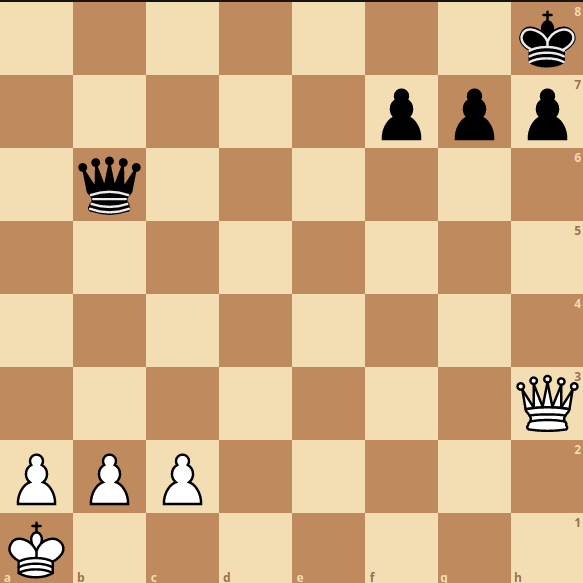
\includegraphics[width=.8\textwidth]{./images/tablero1.png}} 
    \subfigure[]{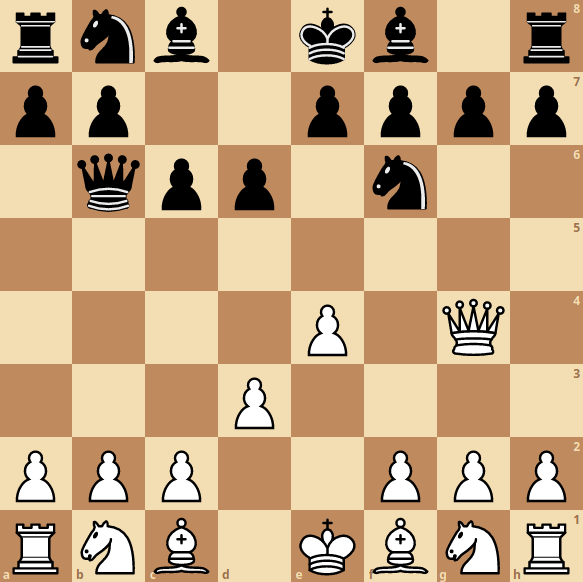
\includegraphics[height=0.45\textwidth]{./images/tablero2.png} 
    \caption{Execution of the eightpuzzle}
    \centering
    \label{8p}
\end{figure}